\documentclass[final]{beamer} % beamer 3.10: do NOT use option hyperref={pdfpagelabels=false} !
 %\documentclass[final,hyperref={pdfpagelabels=false}]{beamer} % beamer 3.07: get rid of beamer warnings
 \mode<presentation> { %% check http://www-i6.informatik.rwth-aachen.de/~dreuw/latexbeamerposter.php for examples 
% \usetheme{Warsaw}
% \usetheme{Aachen}
% \usetheme{Oldi6}
% \usetheme{I6td}
\usetheme{AyuTra}
% \usetheme{I6pd}
% \usetheme{I6pd2}
 }
%\usepackage[htt]{hyphenat}
\usepackage[english]{babel}
\usepackage[utf8]{inputenc}
\usepackage{multirow}
\usepackage{booktabs}
\usepackage{tikz}
\usepackage{pifont}
\usepackage{changepage}
\usepackage{fancybox}
\usepackage{tikz}
\usepackage[pscoord]{eso-pic}% The zero point of the coordinate systemis the lower left corner of the page (the default).
\usetikzlibrary{positioning, shapes}
\definecolor{forrest}{RGB}{34,139,34}
\renewcommand{\baselinestretch}{0.95}

\newcommand{\placetextbox}[3]{% \placetextbox{<horizontal pos>}{<vertical pos>}{<stuff>}
  \setbox0=\hbox{#3}% Put <stuff> in a box
  \AddToShipoutPictureFG*{% Add <stuff> to current page foreground
    \put(\LenToUnit{#1\paperwidth},\LenToUnit{#2\paperheight}){\vtop{{\null}\makebox[0pt][c]{#3}}}%
  }%
}%

\newcommand{\cmark}{\ding{51}}%
\newcommand{\xmark}{\ding{55}}%
\newcommand*\circled[1]{\tikz[baseline=(char.base)]{
            \node[shape=circle,draw,inner sep=2pt] (char) {#1};}}
\newcommand{\mydelta}{$\Delta$\%}
\usepackage{amsmath,amsthm, amssymb, latexsym}
 %\usepackage{times}\usefonttheme{professionalfonts} % times is obsolete
 \usefonttheme[onlymath]{serif}
 \boldmath
 \usepackage[orientation=portrait,size=a0,scale=1.4]{beamerposter} % e.g. for DIN-A0 poster
 %\usepackage[orientation=portrait,size=a1,scale=1.4,grid,debug]{beamerposter} % e.g. for DIN-A1 poster, with optional grid and debug output
%\usepackage[size=custom,width=90,height=150,scale=2.1,debug]{beamerposter} % e.g. for custom size poster
 %\usepackage[orientation=portrait,size=a0,scale=1.0,printer=rwth-glossy-uv.df]{beamerposter} % e.g. for DIN-A0 poster with rwth-glossy-uv printer check
 % ...
 %


\newcommand{\minitab}[2][l]{\begin{tabular}{#1}#2\end{tabular}}
\setbeamertemplate{caption}[numbered]
\newlength{\wideitemsep}
\setlength{\wideitemsep}{\itemsep}
\addtolength{\wideitemsep}{8pt}
\let\olditem\item
\renewcommand{\item}{\setlength{\itemsep}{\wideitemsep}\olditem}
\setbeamertemplate{itemize/enumerate subbody begin}{\vspace{0.8cm}}
\setbeamertemplate{itemize/enumerate subbody end}{\vspace{0.8cm}}
\setbeamersize{text margin left=2.5cm,text margin right=2.5cm}

\addtobeamertemplate{block example begin}{%
  \setlength{\textwidth}{0.95\textwidth}%
}{}

\addtobeamertemplate{block example begin}
  {}
  {\vspace{1ex plus 0.5ex minus 0.5ex} % Pads top of block
     % separates paragraphs in a block
   %\setlength{\parskip}{24pt plus 1pt minus 1pt}%
   \begin{adjustwidth}{1cm}{1cm}
}
\addtobeamertemplate{block example end}
  {\end{adjustwidth}%
   \vspace{1ex plus 0.5ex minus 0.5ex}}% Pads bottom of block
  {\vspace{1ex plus 0.5ex minus 0.5ex}} % Seperates blocks from each other


\title{Apertium: A free/open-source platform \\ for machine translation and basic language technology \\[5mm]
\texttt{www.apertium.org}}
 \author[Forcada, M.L. \& Tyers, F.M.]{\textbf{Mikel L. Forcada$^1$ \and Francis M.\ Tyers$^{2,3}$}}

\institute[mlf@ua.es, ftyers@iu.edu]{$^1$Departament de Llenguatges i Sistemes Inform{\`{a}}tics, Universitat d'Alacant, E-03690 Sant Vicent del Raspeig (Spain) \\ $^2$Department of Linguistics, Indiana University, IN 47405, U.S.A.\\ $^3$ School of Linguistics, Higher School of Economics, Moscow, Russia }
\newcommand{\Pair}[2]{\texttt{#1}\(\leftrightarrow\)\texttt{#2}}
\newcommand{\pair}[2]{\texttt{#1}\(\to\)\texttt{#2}}

\begin{document}

\begin{frame}
\begin{columns}
\begin{column}{0.5\textwidth}

\begin{block}{Apertium components}
\textbf{Since 2005}, Apertium provides:
\begin{enumerate}
\item A free/open-source, modular, shallow/deep transfer, language-independent machine translation \emph{engine} with: text format management, finite-state lexical processing, statistical and constraint-based lexical disambiguation, discontiguous multi-word assembly and disassembly, anaphora resolution, and shallow structural transfer based on finite-state pattern matching 
\item Free/open-source \textbf{linguistic data} in well-specified XML formats for a   variety of languages and language pairs 
\item Free/open-source tools: \textbf{compilers} to turn linguistic
  data into a fast and compact form used by the engine and software to
  learn disambiguation or translation rules from corpora.
\end{enumerate}

Most of the engine developed inside Apertium but some external technologies used: Helsinki Finite-State toolkit (for some morphologically-rich languages), VISL CG-3 (constraint grammars for rule-based lexical disambiguation).

\end{block}

\begin{block}{Machine translation but not only!}

\begin{center}
%  \begin{tabular}{cccccc}
%    \textbf{SL text}$\to$ & \framebox{De-formatter} & & \\
%     & $\downarrow$        & & \\
%     & \framebox{Morphological analyser} & [$\gets$FST] \\
%     & $\downarrow$        & & \\
%     & \framebox{Categorial disambiguator} & [$\gets$FST+stat./ CG rules] \\
%     & $\downarrow$        & & \\
%     & \framebox{Lexical transfer} & [$\gets$FST] \\
%     & $\downarrow$        & & \\
%     & \framebox{Lexical selection} & [$\gets$rules/FST] \\
%     & $\downarrow$        & & \\
%     & \framebox{Structural transfer} &[$\gets$rules] \\
 %    & $\downarrow$        & & \\ 
%     & \framebox{Morphological generator} & [$\gets$FST]   \\
%     & $\downarrow$        & & \\
%      & \framebox{Post-generator} & [$\gets$FST] \\
%     & $\downarrow$        & & \\
%      & \framebox{Re-formatter} & $\to$\textbf{TL text} \\
%  \end{tabular}
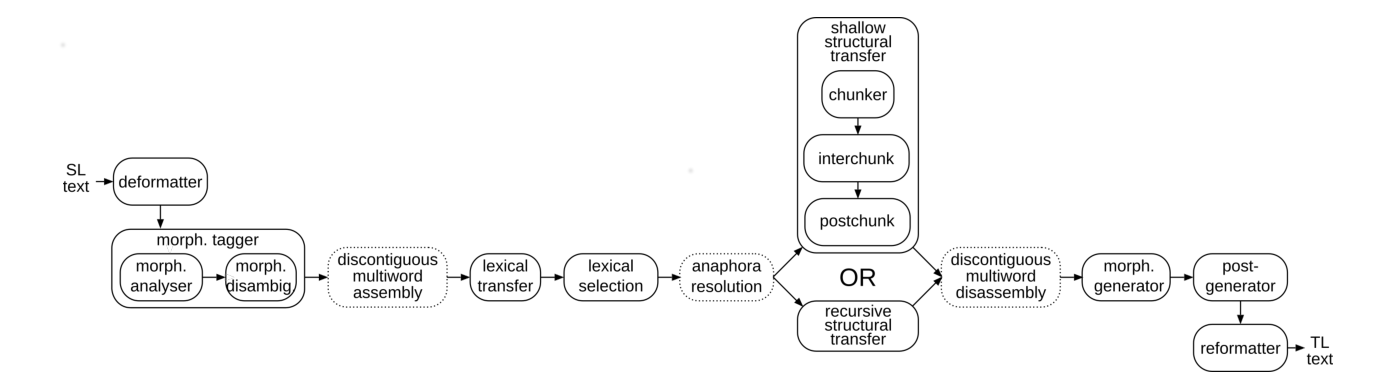
\includegraphics[width=0.95\textwidth]{Images/architecture.pdf}
\end{center}
\begin{itemize}
\item Apertium is a \emph{rule-based machine translation system} but the pipeline contains many \textbf{monolingual} modules that can be used for other human-language technology tasks.
\item Most modules are based on finite-state technology, with HMMs used for part-of-speech tagging and interpreted in the structural transfer.in the structural transfer.
\end{itemize}



\end{block}

\begin{block}{Licensing: free/open-source}
Apertium language data and code are both licensed under the GNU GPL:\begin{itemize}
\item a free/open-source license allowing free distribution of unmodified and modified versions
\item a \textit{copylefted} license: it avoids private appropriation and encourages giving improvements back to the project (a \textit{commons}) \(\to\) \textbf{community}
\end{itemize}
\end{block}

\begin{block}{The Apertium community}
\begin{itemize}
\item Very active group of hundreds of developers 
\item Wiki documentation (\url{wiki.apertium.org})
\item Easy entry: Apertium linguistic modelling is simple, no need to program.
\item IRC channel \url{\#apertium} in \url{freenode.net}
\item Mailing lists: \url{apertium-stuff@lists.sf.net} and other lists
\end{itemize}

\end{block}




\begin{block}{Research and business with Apertium}
  Apertium is already an active research and business platform:
  \begin{itemize}
    \item \textbf{Research:} 40+ publications, 2 PhD thesis, 4 master's theses
    \item \textbf{Business:} companies (Prompsit, Eleka,
      Imaxin Software, etc.) offering services to customers such as
      Autodesk, the Government of Catalonia, one of the main Basque
      banks, the daily newspaper \emph{La Voz de Galicia}, etc.)
  \end{itemize}
  The free/open-source model creates a \textbf{community} which effectively
  connects \textbf{researchers}, \textbf{developers}, \textbf{vendors} and \textbf{users}.
\end{block}

\begin{block}{Ready-to-use Apertium products}
\begin{itemize}\itemsep 0ex
  \item Available as a PPA repository for GNU/Linux users.
  \item Stand-alone applications for the desktop: \texttt{apertium-caffeine} (Java), \textit{Apertium Simpleton} (Windows,MacOS).
  \item an Android version for handhelds
  \item a plug-in for the OmegaT CAT platform \texttt{apertium-omegat}
\end{itemize}
\end{block}

\end{column}
\begin{column}{0.5\textwidth}

\begin{block}{Languages and language pairs}

Language data is encoded mostly in XML, but some language pairs contain data encoded in other text-based formats.

\emph{Stable} language pairs (bilingual data) include: 
\begin{center}
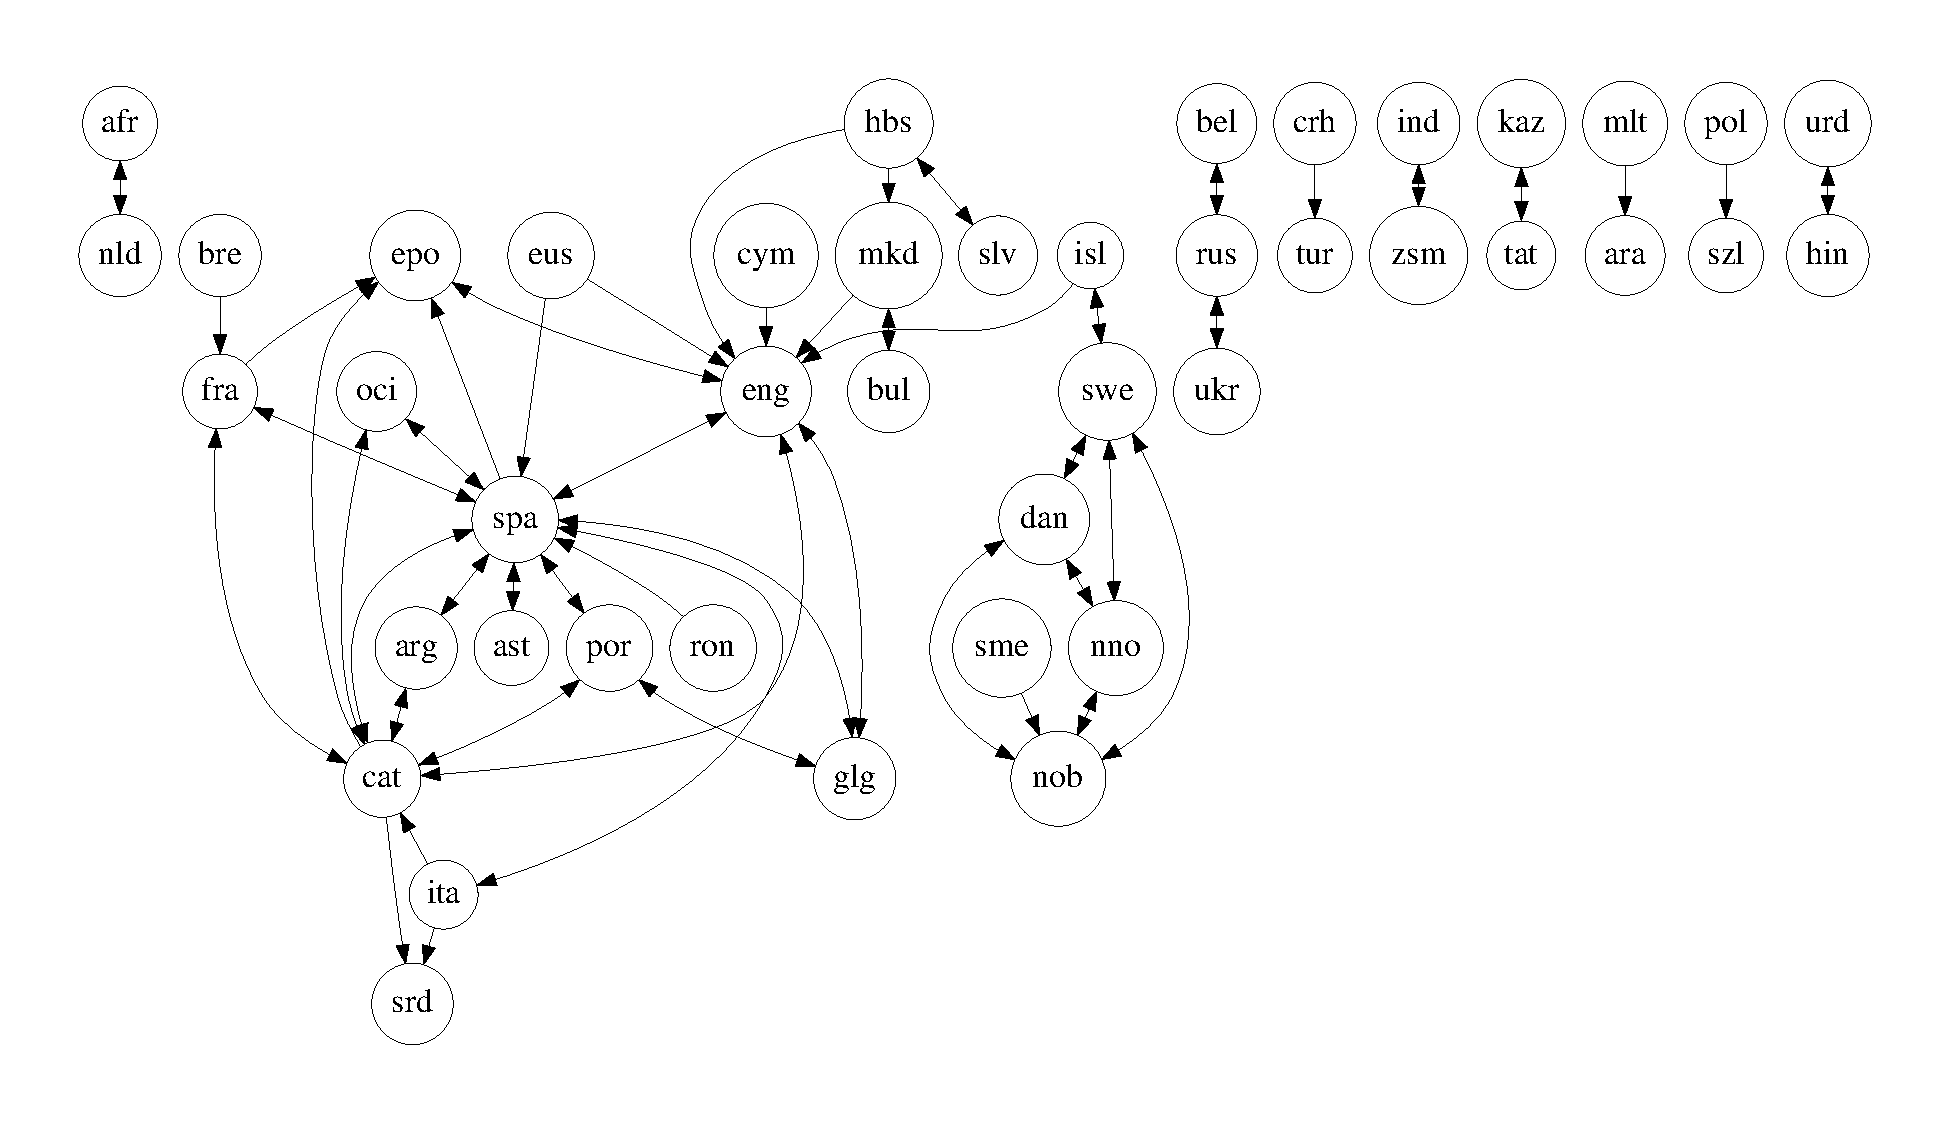
\includegraphics[width=0.82\textwidth]{Images/pairs.pdf}
\end{center}
For many of these languages, there are separate \textit{monolingual} packages.
\end{block}


\begin{block}{Apertium loves small languages}
\begin{tabular}{l}%{p{14cm}}
Some unique MT systems for small languages:
\end{tabular}
\begin{tabular}{lll}
Breton\(\to\)French & Aragonese\(\leftrightarrow\)Spanish & Occitan\(\leftrightarrow\)Catalan  \\
Aragonese\(\leftrightarrow\)Catalan & Occitan\(\leftrightarrow\)Spanish & North Sámi\(\to\)Norwegian \\
Crimean Tatar \(\to\) Turkish & ~ & ~ \\
\end{tabular}
\end{block}





\begin{block}{Success cases}
Apertium is used:
\flushright	
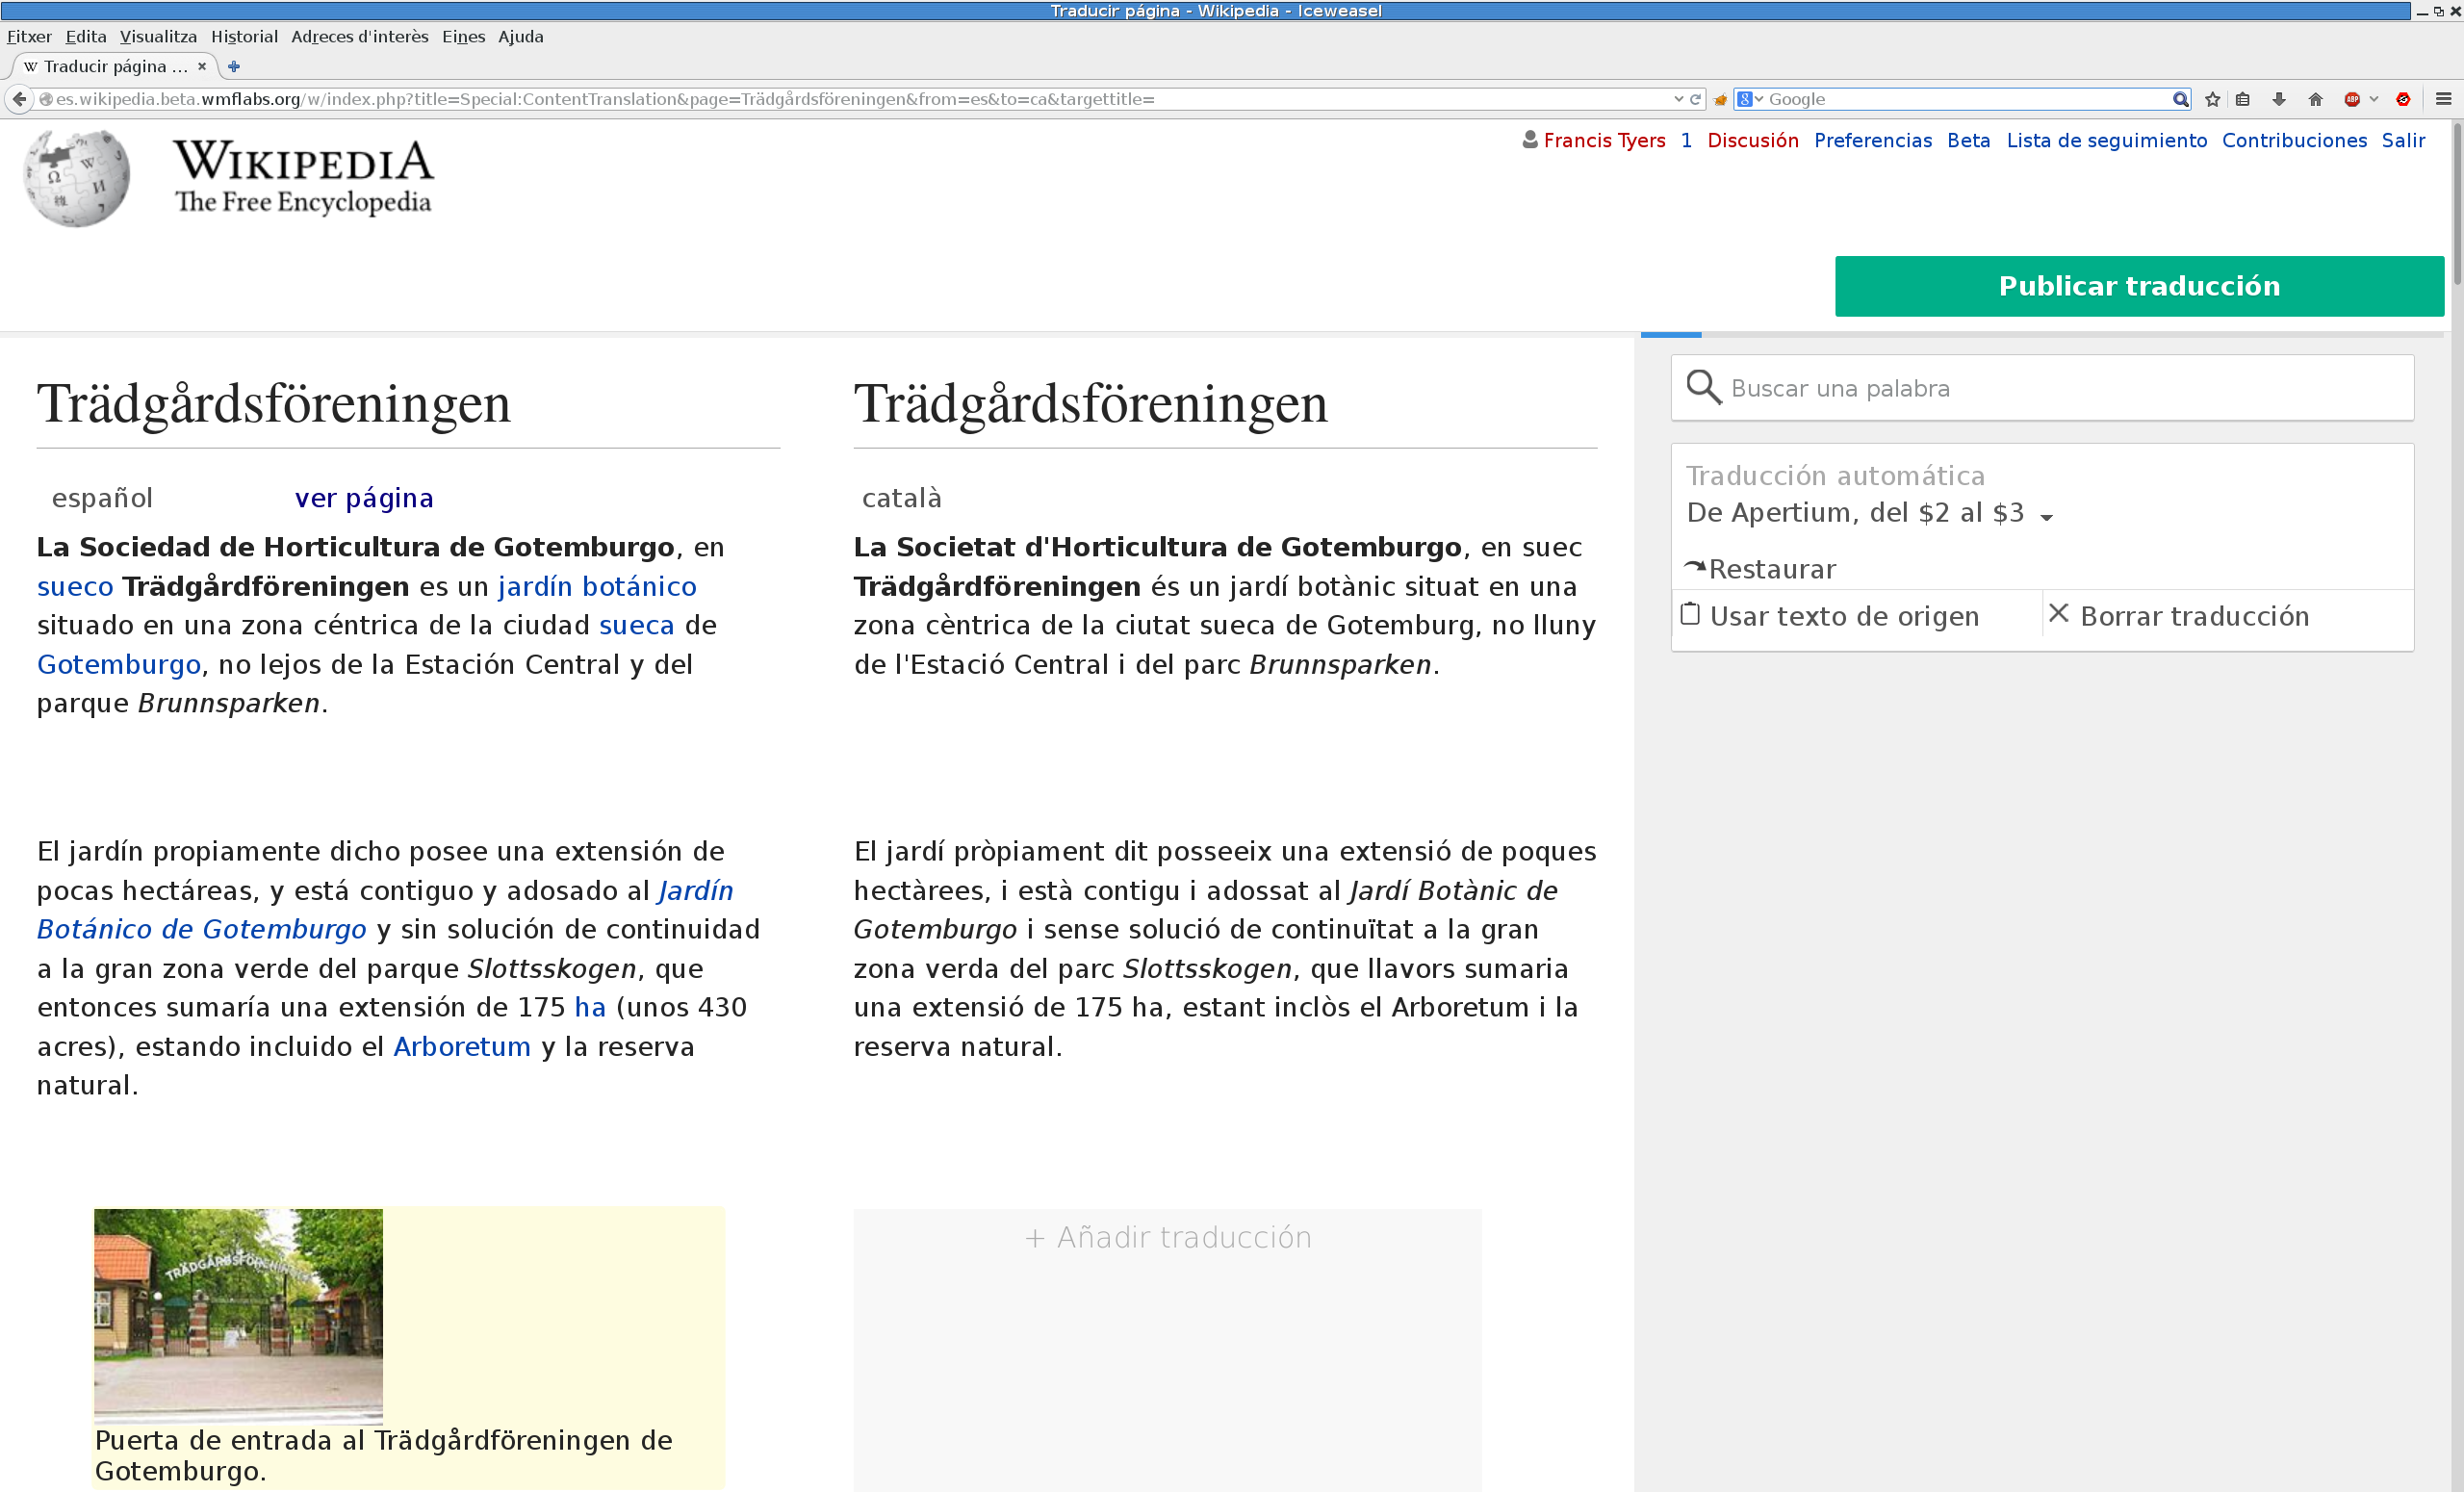
\includegraphics[width=0.84\textwidth]{Images/captura-mediawiki.png}
\flushleft
\begin{itemize}
\item in Wikimedia Content Translation to generate Wikipedia content,
\item to produce a Catalan edition of Valencia daily newspaper \textit{Levante-EMV},
\item by Universities in the Catalan speaking area to help in the generation of courseware and academic information,
\item in PLATA, the Spanish government platform for webpage machine translation.
\end{itemize}
\end{block}

\begin{block}{Funding}
\begin{itemize}
\item The Ministry of Industry, Tourism and Commerce of Spain (also,
  the Ministries of Education and Science and of Science
  and Technology of Spain)
\item The Secretariat for Technology and the Information Society of the Government of Catalonia
\item The European Commission (Abu-Matran project)
\item The Ministry of Foreign Affairs of Romania
\item Universitat d'Alacant and Universitat Oberta de Catalunya
\item Ofis Publik ar Brezhoneg (Breton Language Board)
\item Google Summer of Code scholarships (2009--2014, 2016) and Google Code-In donations.
\item Companies: Prompsit Language Engineering, ABC Enciklopedioj, Eleka Ingeniartiza Linguistikoa, imaxin|software, Eolaistriu Technologies, Kaldera, etc.

\end{itemize} 
\end{block}


\end{column}
\end{columns}
\end{frame}
\end{document}

\begin{columns}
\begin{column}{1.01\textwidth}
\vbox to .115\textheight{

    \begin{block}{%{\LARGE \ding{182}} 
    1~~Word-level MT quality estimation}

\begin{columns}
 \begin{column}{.58\textwidth}

\textbf{The problem}: detecting which words in the MT output (\(\mathrm{MT}(S)\)) should be post-edited
\vspace{0.5cm}
   \begin{exampleblock}{}
    \begin{center}
	\(S\)=``l'Associació Europea per a la Traducció Automàtica''

	\(\mathrm{MT}(S)\)=``\textcolor{forrest}{the European Association for} \textcolor{red}{the Automatic} \textcolor{forrest}{Translation}''

	\(T\)=``the European Association for Machine Translation''
    \end{center}
   \end{exampleblock}

\end{column}
 \begin{column}{.38\textwidth}

\textbf{Useful for:}
\begin{itemize}
  \setlength{\itemindent}{1em}
 \item estimating post-editing effort and budgeting translation
 \item choosing among alternative translations
 \item guiding post-editing
\end{itemize}
\phantom{a}

\end{column}
\end{columns}

\end{block}
   }

\end{column}
\end{columns}

\begin{columns}
 \begin{column}{.49\textwidth}


\vbox to .49\textheight{%

    \begin{block}{{\LARGE \ding{183}} Our approach}
     
     Our approach uses \textbf{any source of bilingual information (SBI)} that allows to translate segments (e.g. MT, bilingual concordancers, dictionaries, etc.) by:
\vspace{-1cm}
	 \begin{enumerate}
  \setlength{\itemindent}{2em}
	  \item obtaining all the possible sub-segments \(\sigma\) from both \(S\) and \(\tau\) from \(\mathsf{MT}(S)\), up to a given length \(L\) in both sides (\(L=3\) in the example):
\begin{columns}[t]
\begin{column}{0.04\textwidth}
\end{column}
\begin{column}{0.96\textwidth}
   \begin{exampleblock}{}
     \textbf{\(\sigma\) (Catalan)}

     l'

     l' Associació

     l' Associació Europea

     ...

     la Traducció Automàtica
   \end{exampleblock}

\end{column}
\end{columns}

	  \item translating them (in both directions) with any available source of bilingual information to obtain \((\sigma,\tau)\) pairs

\begin{columns}[t]
\begin{column}{0.04\textwidth}
\end{column}
\begin{column}{0.96\textwidth}     \begin{exampleblock}{}
     \textbf{\(\sigma\) (Catalan) $\rightarrow$ \(\tau\) (English)}

     l' $\rightarrow$ the

     l' Associació $\rightarrow$ the Association

     l' Associació Europea $\rightarrow$ the European Association

     ...

     la Traducció Automàtica $\rightarrow$ the Machine Translation
   \end{exampleblock}
\end{column}
\end{columns}

	  \item for those sub-segment pairs \((\sigma,\tau)\) for which \(\sigma\) matches \(S\): matching (totally or partially) the \(\tau\) sub-segments with $\mathsf{MT}(S)$

\begin{columns}[t]
\begin{column}{0.04\textwidth}
\end{column}
\begin{column}{0.96\textwidth}     \begin{exampleblock}{}



	\(\mathrm{MT}(S)\)=``the European Association for the Automatic Translation''

\hspace*{5.1cm} \, \cmark \:\:\:\:\:\:\:\: \cmark \:\:\:\:\:\:\:\:\:\:\:\:\:\:\:\: \cmark  \hspace*{3.6cm} \, \cmark \:\:\:\:\:\:\:\:\:\: \xmark \:\:\:\:\:\:\:\:\:\:\:\:\:\:\:\: \cmark

\hspace*{5.4cm} \textcolor{forrest}{the European Association}  \hspace*{1.1cm} \textcolor{forrest}{the} \: \textcolor{red}{Machine}\,\, \textcolor{forrest}{Translation}
   \end{exampleblock}
\end{column}
\end{columns}

	  \item extracting a collection of positive and negative features for each source of bilingual information and for each translation direction that represents matching information for $\mathsf{MT}(S)$, and using a neural network binary classifier



	 \end{enumerate}

\end{block}


}


\vbox to .44\textheight{%
 \begin{block}{{\LARGE \ding{184}} Features}
   \textbf{Positive features} use those sub-segment pairs \((\sigma,\tau)\) for which, \(\tau\) fully matches in \(\mathrm{MT}(S)\):
   \begin{center}

    \begin{exampleblock}{}

\placetextbox{0.168}{0.29}{\texttt{\textcolor{blue}{\(\sigma\)}}}%

	\hspace*{3cm} \(S\) = ``\underline{\textcolor{blue}{l'Associació Europea}} per a la Traducció Automàtica''

\begin{tikzpicture}[font=\large\sffamily]
%\node [rotate=-135] at (17.4cm, 9cm) {{\Huge \(\curvearrowright\)}};
%\hspace*{3.5cm} \node[cloud, cloud puffs=20, cloud ignores aspect, minimum width=3cm, minimum height=1cm, align=left, draw] (cloud) at (9cm, 9cm) {\small translate \textcolor{blue}{\(\sigma\)} with SBI};
%\node [rotate=45] at (3.8cm, 9cm) {{\Huge \(\curvearrowleft\)}};
\node [rotate=-135] at (15.7cm, 9cm) {{\Huge \(\curvearrowright\)}};
\hspace*{1cm} \node[cloud, cloud puffs=20, cloud ignores aspect, minimum width=3cm, minimum height=1cm, align=left, draw] (cloud) at (7.2cm, 9cm) {\small translate \textcolor{blue}{\(\sigma\)} with SBI};
\node [rotate=45] at (0cm, 9cm) {{\Huge \(\curvearrowleft\)}};

\end{tikzpicture}

        %\hspace*{3cm} \(\sigma\) = ``l' Associació Europea''

        \hspace*{3cm} \(\tau\) = ``the European Association''

        \hspace*{6cm} \, \cmark \:\:\:\:\:\:\:\: \cmark \:\:\:\:\:\:\:\:\:\:\:\:\:\:\:\: \cmark

	\(\mathrm{MT}(S)\) = ``\underline{\textcolor{forrest}{the European Association}} for the Automatic Translation''

  \end{exampleblock}
 \end{center}

\vspace{-0.7cm}

   \emph{Translation frequencies} are available for some sources of bilingual information (such as bilingual concordancers); they are used to produce a \emph{weighted} version of the positive features

\vspace{1cm}

   \textbf{Negative features} use those sub-segment pairs \((\sigma,\tau)\) for which \(\tau\) does not match \(\mathrm{MT}(S)\), but such that the beginning and the ending of \(\tau\) can be aligned to \(\mathrm{MT}(S)\), therefore indicating possible deletions or substitutions


   \begin{center}
    \begin{exampleblock}{}

\placetextbox{0.33}{0.099}{\texttt{\textcolor{blue}{\(\sigma\)}}}%

	\hspace*{3cm} \(S\) = ``l'Associació Europea per a \underline{\textcolor{blue}{la Traducció Automàtica}}''

\begin{tikzpicture}[font=\large\sffamily]
\node [rotate=-135] at (29.4cm, 9cm) {{\Huge \(\curvearrowright\)}};
\hspace*{14cm} \node[cloud, cloud puffs=20, cloud ignores aspect, minimum width=3cm, minimum height=1cm, align=left, draw] (cloud) at (7.8cm, 9cm) {\small translate \textcolor{blue}{\(\sigma\)} with SBI};
\node [rotate=45] at (0.1cm, 9cm) {{\Huge \(\curvearrowleft\)}};

\end{tikzpicture}

        %\hspace*{3cm} \(\sigma\) = ``l' Associació Europea''

        \hspace*{16.3cm} \(\tau\) = the \: Machine\,\, Translation

        \hspace*{18.4cm} \, \cmark \:\:\:\:\:\:\:\:\:\:\: \xmark \:\:\:\:\:\:\:\:\:\:\:\:\:\:\:\: \cmark

	\(\mathrm{MT}(S)\) = ``the European Association \underline{\textcolor{forrest}{the} \textcolor{red}{Automatic} \textcolor{forrest}{Translation}}''

  \end{exampleblock}
 \end{center}



\end{block}
   }


  \end{column}

 \begin{column}{.49\textwidth}
 



\vbox to .315\textheight{%
 \begin{block}{{\LARGE \ding{185}} Experiments}

\textbf{Data sets:} English segments (\(S\)) translated into Spanish (\(\mathrm{MT}(S)\)) with MTQE labels (``GOOD'' and ``BAD'') and a collection of \textbf{baseline} features:

 \begin{table}
     \centering
     \begin{tabular}{lp{1cm}rp{1cm}cp{1cm}c}
       \toprule
       \textbf{data set} & & \textbf{size} & & \textbf{baseline features} & & \textbf{MTQE labels} \\ \midrule
       training    & & 11,272 & & \cmark & & \cmark \\
       development & &  1,000 & & \cmark & & \cmark \\
       test        & &  1,817 & & \cmark & & \xmark \\
       \hline \bottomrule
     \end{tabular}
  \end{table}

\vspace{1cm}

\textbf{Binary classification}: \emph{multilayer perceptron}, one layer, as many neurons as features; 10\% of the training set used as a validation set; development set used for hiperparameter optimisation

\vspace{1cm}

\textbf{Evaluation metrics}: precision ($P$), recall ($R$), F-score ($F_1$), and weighted F-score (\(F_1^w\)).

\vspace{1cm}

\textbf{Sources of bilingual information} used:
\begin{itemize}
  \setlength{\itemindent}{2em}
 \item \emph{Reverso Context}: bilingual concordancer, many translation suggestions for each \(\sigma\), translation frequency available  (\url{http://context.reverso.net})
 \item \emph{Machine translation}: Apertium (\url{http://www.apertium.org}) and Google Translate (\url{http://translate.google.com}) MT systems, only one translation suggestion for each \(\sigma\), translation frequency not available
\end{itemize}


\end{block}
   }


\vbox to .27\textheight{%

    \begin{block}{%{\LARGE \ding{186}} 
    5~~Results}
       
Results on the \textbf{development set}:

\vspace{-1cm}

 \begin{table}
          \centering
        \begin{tabular}{lp{1cm}rrrp{1cm}rrrp{1cm}r}
        \toprule
        \textbf{System} & & $P^{\mathrm{BAD}}$ & $R^{\mathrm{BAD}}$ & $F_1^{\mathrm{BAD}}$ & & $P^{\mathrm{GOOD}}$ & $R^{\mathrm{GOOD}}$ & $F_1^{\mathrm{GOOD}}$ & & $F_1^{w}$ \\ \midrule
        SBI          & & 31.2\% & 63.7\% & 41.9\% & & 88.5\% & 66.7\% & 76.1\% & & 69.5\% \\ \vspace{2mm}
        SBI+baseline & & 33.4\% & 60.9\% & 43.1\% & & 88.5\% & 71.1\% & 78.8\% & & 72.0\% \\
        \hline \bottomrule
        \end{tabular}
        \label{tb:results}

        \end{table}

Results on the \textbf{test set}:

\vspace{-1cm}

       \begin{table}
          \centering
        \begin{tabular}{lp{1cm}rrrp{1cm}rrrp{1cm}r}
        \toprule
        \textbf{System} & & $P^{\mathrm{BAD}}$ & $R^{\mathrm{BAD}}$ & $F_1^{\mathrm{BAD}}$ & & $P^{\mathrm{GOOD}}$ & $R^{\mathrm{GOOD}}$ & $F_1^{\mathrm{GOOD}}$ & & $F_1^{w}$ \\ \midrule
        baseline     & &  ---   &  ---   & 16.8\% & &  ---   &  ---   & 88.9\% & & 75.3\% \\
        SBI          & & 30.8\% & 63.9\% & 41.5\% & & 88.8\% & 66.5\% & 76.1\% & & 69.5\% \\
        SBI+baseline & & 32.6\% & 63.6\% & 43.1\% & & 89.1\% & 69.5\% & 78.1\% & & 71.5\% \\
        \hline \bottomrule
        \end{tabular}
        \label{tb:results}

        \end{table}

  \begin{itemize}
   \item \emph{baseline:} organizers' baseline using linear regression classification on the baseline features
   \item \emph{SBI:} using only features from sources of bilingual information
   \item \emph{SBI+baseline:} combining features from sources of bilingual information and baseline features
  \end{itemize}

    \end{block}
}

\vbox to .125\textheight{%
    \begin{block}{{\LARGE \ding{187}} Highlights}
  \begin{itemize}
   \item SBI system ranked \textbf{3rd} and SBI+baseline system ranked \textbf{1st} in the task
   \item Our system uses only online available sources of bilingual information
   \item The method is \textbf{system independent}: can be used on any kind of MT system output
   \item Any \textbf{other sources of bilingual information} can be easily added
  \end{itemize}

    \end{block}
}

\vbox to .215\textheight{%
\begin{block}{Acknowledgements}


We specially thank \textbf{Reverso-Softissimo} and \textbf{Prompsit Language Engineering} for providing
  the access to the Reverso Context concordancer, and the \textbf{University Research Program
  for Google} Translate for providing the access to Google Translate

\vspace{1cm}

 Work partially funded by:
            \begin{figure}
              \centering
              \includegraphics[scale=0.54]{Images/logo_Marie_Curie_Actions.jpg} \hspace{3cm}
              \includegraphics[scale=1.3]{Images/Logotipo_del_Ministerio_de_Ciencia.png}
            \end{figure}
 %\begin{itemize}
 % \setlength{\itemindent}{1em}
 % \item Spanish government, project TIN2012-32615 (AyuTra)
 % \item European Commission, project PIAP-GA-2012-324414 (Abu-MaTran)
 %\end{itemize}

\end{block}
}
\end{column}

\end{columns}



\end{frame}
\end{document}
